% fig_coverage_heatmap.tex -- results example: tab:coverage redrawn as an
% actual heatmap figure rather than a text/color table. Same real numbers
% as main.tex's Table 1 (tab:coverage): 3 models x 6 axes, trackability %.
% Draft only, not wired into main.tex -- a faster-to-read companion or
% talk-slide substitute for the table.

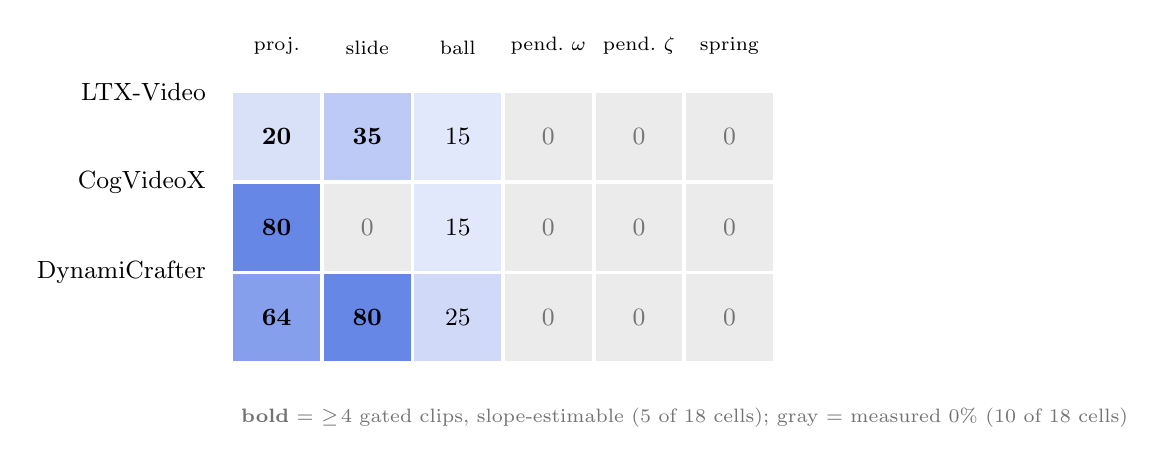
\begin{tikzpicture}[font=\small]

\def\models{{LTX-Video},{CogVideoX},{DynamiCrafter}}
\def\axes{{proj.},{slide},{ball},{pend.\ $\omega$},{pend.\ $\zeta$},{spring}}
\def\cellsize{1.15}

\foreach [count=\r from 0] \modelrow in \models {
  \node[font=\small,anchor=east] at (-0.2,{-\r*\cellsize}) {\modelrow};
}
\foreach [count=\c from 0] \axisname in \axes {
  \node[font=\scriptsize,anchor=south,align=center,rotate=0] at ({\c*\cellsize+\cellsize/2},0.35) {\axisname};
}

% Row 0: LTX-Video
\foreach [count=\c] \v/\bold in {20/1,35/1,15/0,0/0,0/0,0/0} {
  \pgfmathsetmacro{\x}{(\c-1)*\cellsize}
  \pgfmathsetmacro{\y}{0}
  \pgfmathsetmacro{\shade}{\v}
  \ifnum\bold=1
    \fill[RoyalBlue!\shade!white] (\x,-\y) rectangle ++(\cellsize,-\cellsize);
    \node[font=\small\bfseries,text=black] at ({\x+\cellsize/2},{-\y-\cellsize/2}) {\v};
  \else
    \ifnum\v=0
      \fill[black!8] (\x,-\y) rectangle ++(\cellsize,-\cellsize);
      \node[font=\small,text=black!55] at ({\x+\cellsize/2},{-\y-\cellsize/2}) {0};
    \else
      \fill[RoyalBlue!\shade!white] (\x,-\y) rectangle ++(\cellsize,-\cellsize);
      \node[font=\small,text=black] at ({\x+\cellsize/2},{-\y-\cellsize/2}) {\v};
    \fi
  \fi
  \draw[white,line width=1.4pt] (\x,-\y) rectangle ++(\cellsize,-\cellsize);
}
% Row 1: CogVideoX
\foreach [count=\c] \v/\bold in {80/1,0/0,15/0,0/0,0/0,0/0} {
  \pgfmathsetmacro{\x}{(\c-1)*\cellsize}
  \pgfmathsetmacro{\y}{\cellsize}
  \pgfmathsetmacro{\shade}{\v}
  \ifnum\bold=1
    \fill[RoyalBlue!\shade!white] (\x,-\y) rectangle ++(\cellsize,-\cellsize);
    \node[font=\small\bfseries,text=black] at ({\x+\cellsize/2},{-\y-\cellsize/2}) {\v};
  \else
    \ifnum\v=0
      \fill[black!8] (\x,-\y) rectangle ++(\cellsize,-\cellsize);
      \node[font=\small,text=black!55] at ({\x+\cellsize/2},{-\y-\cellsize/2}) {0};
    \else
      \fill[RoyalBlue!\shade!white] (\x,-\y) rectangle ++(\cellsize,-\cellsize);
      \node[font=\small,text=black] at ({\x+\cellsize/2},{-\y-\cellsize/2}) {\v};
    \fi
  \fi
  \draw[white,line width=1.4pt] (\x,-\y) rectangle ++(\cellsize,-\cellsize);
}
% Row 2: DynamiCrafter
\foreach [count=\c] \v/\bold in {64/1,80/1,25/0,0/0,0/0,0/0} {
  \pgfmathsetmacro{\x}{(\c-1)*\cellsize}
  \pgfmathsetmacro{\y}{2*\cellsize}
  \pgfmathsetmacro{\shade}{\v}
  \ifnum\bold=1
    \fill[RoyalBlue!\shade!white] (\x,-\y) rectangle ++(\cellsize,-\cellsize);
    \node[font=\small\bfseries,text=black] at ({\x+\cellsize/2},{-\y-\cellsize/2}) {\v};
  \else
    \ifnum\v=0
      \fill[black!8] (\x,-\y) rectangle ++(\cellsize,-\cellsize);
      \node[font=\small,text=black!55] at ({\x+\cellsize/2},{-\y-\cellsize/2}) {0};
    \else
      \fill[RoyalBlue!\shade!white] (\x,-\y) rectangle ++(\cellsize,-\cellsize);
      \node[font=\small,text=black] at ({\x+\cellsize/2},{-\y-\cellsize/2}) {\v};
    \fi
  \fi
  \draw[white,line width=1.4pt] (\x,-\y) rectangle ++(\cellsize,-\cellsize);
}

\node[font=\scriptsize,black!55,anchor=north west,align=left] at (0,-3.9)
  {\textbf{bold} = $\ge\!4$ gated clips, slope-estimable (5 of 18 cells);
   gray = measured $0\%$ (10 of 18 cells)};

\end{tikzpicture}
